%
% NOTE -- ONLY EDIT THE .Rnw FILE!!!  The .tex file is
% likely to be overwritten.
%
%\VignetteDepends{graph,Rgraphviz}
%\VignetteKeywords{Protein Complex, Graphs}
%\VignettePackage{apComplex}
%\VignetteIndexEntry{apComplex}

\documentclass[11pt]{article}


\usepackage{amsmath,pstricks}
\usepackage[authoryear,round]{natbib}
\usepackage{hyperref}
\usepackage{times}
\usepackage{comment}


\textwidth=6.2in
\textheight=8.5in
%\parskip=.3cm
\oddsidemargin=.1in
\evensidemargin=.1in
\headheight=-.3in

\newcommand{\scscst}{\scriptscriptstyle}
\newcommand{\scst}{\scriptstyle}

\newcommand{\Rfunction}[1]{{\texttt{#1}}}
\newcommand{\Robject}[1]{{\texttt{#1}}}
\newcommand{\Rpackage}[1]{{\textit{#1}}}


\bibliographystyle{plainnat}

\title{Protein complex membership estimation using \Rpackage{apComplex}}
\author{Denise Scholtens}
\date{}

\usepackage{/home/denise/R-2.1.0/share/texmf/Sweave}
\begin{document}
\maketitle
\Rpackage{apComplex} contains functions for estimating protein complex membership using data from
affinity-purification/mass-spectrometry (AP-MS) experiments.  Users must
specify the believed sensitivity and specificity of the AP-MS technology and
may incorporate external similarity data for the proteins under
investigation.  The statistical details of the algorithm are reported in
Scholtens and Gentleman (2004) and the biological implications are discussed
in Scholtens, Vidal, and Gentleman (submitted).  

\begin{Schunk}
\begin{Sinput}
> library(apComplex)
\end{Sinput}
\begin{Soutput}
Loading required package: graph
Loading required package: cluster
Loading required package: Ruuid
Loading required package: Biobase
Welcome to Bioconductor 
	 Vignettes contain introductory material.  To view, 
	 simply type: openVignette() 
	 For details on reading vignettes, see
	 the openVignette help page.
\end{Soutput}
\end{Schunk}

\section*{AP-MS Data}

AP-MS technology is designed to detect complex comembership among proteins.  A
set of proteins are used as baits, and in each purification, the bait protein finds the set of hit proteins with which it
shares membership in at least one complex.  Suppose proteins $P_{1}$, $P_{2}$, $P_{4}$,
and $P_{6}$ compose one complex and proteins $P_{3}$, $P_{4}$ and
$P_{5}$ compose a separate complex.  If proteins $P_{1}$, $P_{2}$, and $P_{3}$
are used as baits, then with perfectly sensitive and specific AP-MS
technology, the following data should be observed.

\vspace{.2in}

\begin{tabular}{cc|cccccc}
 & \multicolumn{1}{c}{} & \multicolumn{6}{c}{Hits} \\
 & \multicolumn{1}{c}{} & $P_{1}$ & $P_{2}$ & $P_{3}$ & $P_{4}$ & $P_{5}$ & $P_{6}$  \\
\cline{3-8}
 & $P_{1}$ & 1 & 1 & 0 & 1 & 0 & 1 \\
Baits & $P_{2}$ & 1 & 1 & 0 & 1 & 0 & 1 \\
 & $P_{3}$ & 0 & 0 & 1 & 1 & 1 & 0 \\
\end{tabular}

\vspace{.2in}

\noindent The rows of the matrix are baits, the columns are hits, an
entry of 1 in the $i$th row and $j$th column indicates that bait protein $i$
finds protein $j$ as a hit, and an entry of 0 in the $i$th row and $j$th
column indicates that bait protein $i$ does not find protein $j$ as a hit.
 The diagonal entries are 1 since a protein is always a complex comember with itself.  Note that bait proteins can be found as hits by other bait
proteins.  Also note that some proteins are never used as baits.  

A graph of the data is useful for understanding which comembership relationships are
tested in AP-MS experiments and which are not.  In the graph in Figure \ref{fig:trueData}, nodes
represent proteins and directed edges from baits to hits represent complex
comembership.  Bait proteins are yellow and hit-only proteins
(i.e. proteins that are found as hits but never used as baits) are white.
Directed edges always originate at yellow bait proteins and point to the set
of hits detected by that bait.  The
red reciprocated edge connecting $P_{1}$ and $P_{2}$ represents a bait-bait relationship that is tested
twice, once in each purification.  The gray unreciprocated edges represent bait-hit-only edges that are
only tested once.  Missing edges between baits and other baits or hit-only
proteins represent comemberships that are tested, but not observed.  Edges
between hit-only proteins are always missing, not because the comemberships
are known not to exist, but because they are never tested.


\begin{figure}[htbp]
\begin{center}
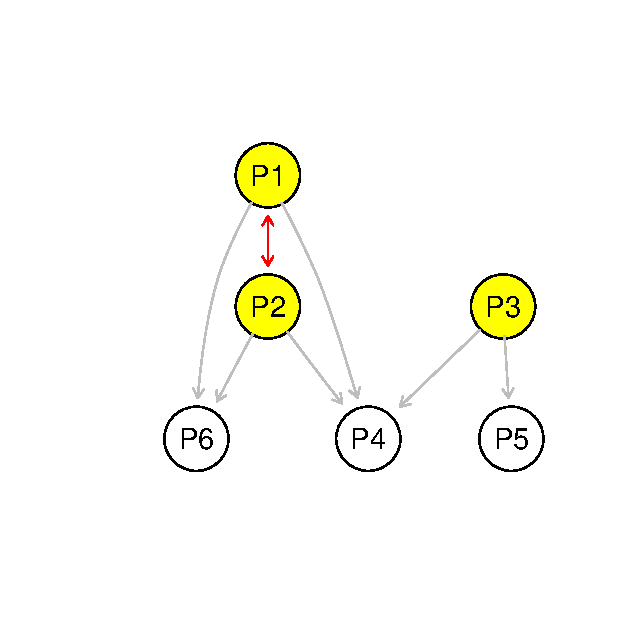
\includegraphics[width=0.5\textwidth]{apComplex-trueData}
\caption{\label{fig:trueData} True complex comemberships that would be
detected with perfectly sensitive and specific AP-MS technology using $P_{1}$,
$P_{2}$, and $P_{3}$ as baits.}
\end{center}
\end{figure}

In reality, AP-MS technology is neither perfectly sensitive nor specific,
resulting in false positive (FP) and false negative (FN) observations of
the complex comemberships under investigation.
Suppose in this experiment, we make a FN observation between $P_{2}$ and
$P_{4}$, i.e. $P_{4}$ is not found as a hit when we use $P_{2}$ as a bait.
Also suppose we make two FP observations: 1) when we use $P_{3}$
as a bait, we find an extraneous hit-only protein $P_{7}$, and 2) when performing
a purification using $P_{8}$ as a bait, we find $P_{3}$ as a hit.
Data for this example are contained in the matrix \Robject{apEX}.  In this
matrix, rows again represent baits and columns represent hits.


\begin{Schunk}
\begin{Sinput}
> data(apEX)
> apEX
\end{Sinput}
\begin{Soutput}
   P1 P2 P3 P8 P4 P5 P6 P7
P1  1  1  0  0  1  0  1  0
P2  1  1  0  0  0  0  1  0
P3  0  0  1  0  1  1  0  1
P8  0  0  1  1  0  0  0  0
\end{Soutput}
\end{Schunk}

The graph of the data in Figure \ref{fig:observedData} demonstrates the observations recorded in \Robject{apEX}.
Note the missing edge from $P_{2}$ to $P_{4}$ and the new edge from $P_{3}$ to
$P_{7}$.  Also note the blue
unreciprocated edge between $P_{3}$ and $P_{8}$ -- this is a complex
comembership that was tested twice when $P_{3}$ and $P_{8}$ were used as baits, but
only detected once in the purification using $P_{8}$ as a bait.



\begin{figure}[htbp]
\begin{center}
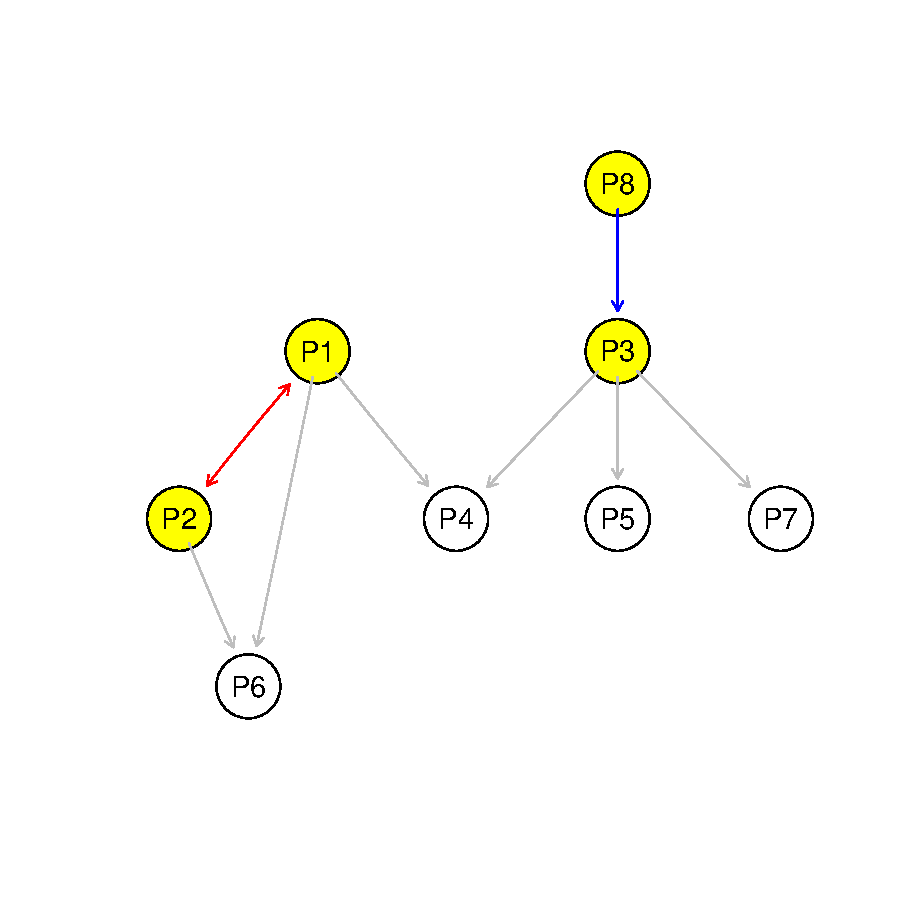
\includegraphics[width=0.5\textwidth]{apComplex-observedData}
\caption{\label{fig:observedData} Hypothetical data from an AP-MS experiment
with a FN observation between $P_{2}$ and $P_{6}$ and FP observations 
between $P_{3}$ and $P_{7}$ and $P_{8}$ and $P_{3}$.}
\end{center}
\end{figure}

\Rpackage{apComplex} starts with observed complex \textit{comembership} data
from AP-MS and estimates complex \textit{membership}.

\section*{Algorithm}

The edges in an AP-MS graph represent complex comembership.  If all proteins
were used as baits, then maximal
complete subgraphs (or cliques) in the AP-MS graph would contain entire collections of proteins that
compose a complex.  The maximal complete subgraphs could then be used to form a protein complex
membership graph (PCMG): a bipartite graph in which one set of nodes
represents proteins, the other set represents complexes, and an edge from a
protein node to a complex node represents membership of the protein in that
complex.  Bipartite graphs can also be represented using an affiliation
matrix in which the rows represent proteins, the columns represent
complexes, and an entry of 1 in the $j$th row and $i$th column represents
membership of protein $i$ in complex $j$.  \Rpackage{apComplex} is essentially a maximal complete
subgraph finding algorithm that is adapted for the bait/hit status of
proteins, as well as imperfect observation of edges.

The first step in estimating complex membership is to find the \textit{maximal
BH-complete subgraphs} in the observed AP-MS data.  A \textit{BH-complete
subgraph} is defined to be a collection of baits and hits for which all bait-bait edges and
all bait-hit-only edges exist; a \textit{maximal BH-complete subgraph} is a
BH-complete subgraph that is not contained in any other BH-complete subgraph.  In the event of unreciprocated observations
between pairs of baits, the edges are estimated to exist when the sensitivity
of the AP-MS technology is less than the specificity.  Under a logistic
regression model where the parameters represent sensitivity and specificity, this treatment of unreciprocated bait-bait edges
maximizes the likelihood $L$ for the data (Scholtens and Gentleman, 2004).  In our example, the observed data contains four maximal
BH-complete subgraphs, shown in Figure \ref{fig:PCMG0}.  The function
\Rfunction{bhmaxSubgraph} will detect these maximal BH-complete subgraphs and
report them using an affiliation matrix.  Figure \ref{fig:BP1}
shows the corresponding bipartite PCMG for the initial complex estimates.

\begin{Schunk}
\begin{Sinput}
> PCMG0 <- bhmaxSubgraph(apEX)
> PCMG0
\end{Sinput}
\begin{Soutput}
   bhmax1 bhmax2 bhmax3 bhmax4
P1      0      1      1      0
P2      0      1      0      0
P3      1      0      0      1
P8      1      0      0      0
P4      0      0      1      1
P5      0      0      0      1
P6      0      1      1      0
P7      0      0      0      1
\end{Soutput}
\end{Schunk}



\begin{figure}[htbp]
\begin{center}
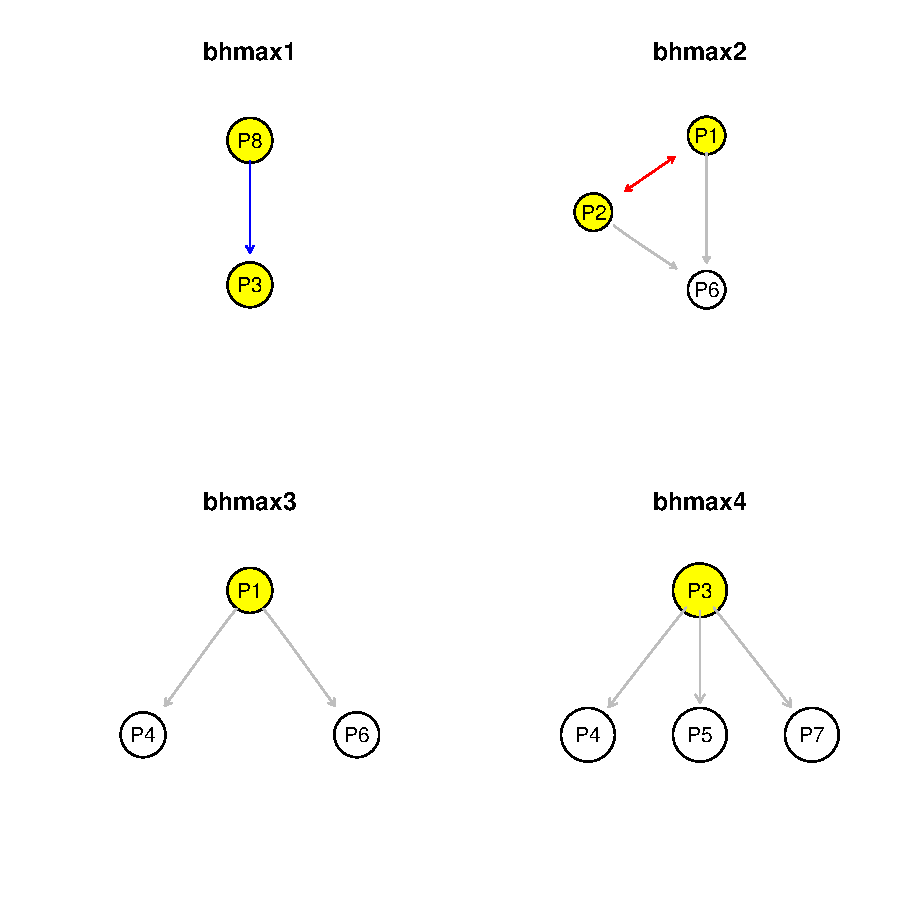
\includegraphics[width=0.6\textwidth]{apComplex-PCMG0graph}
\caption{\label{fig:PCMG0} Four maximal BH-complete subgraphs in the observed
data.}
\end{center}
\end{figure}


\begin{figure}[htbp]
\begin{center}
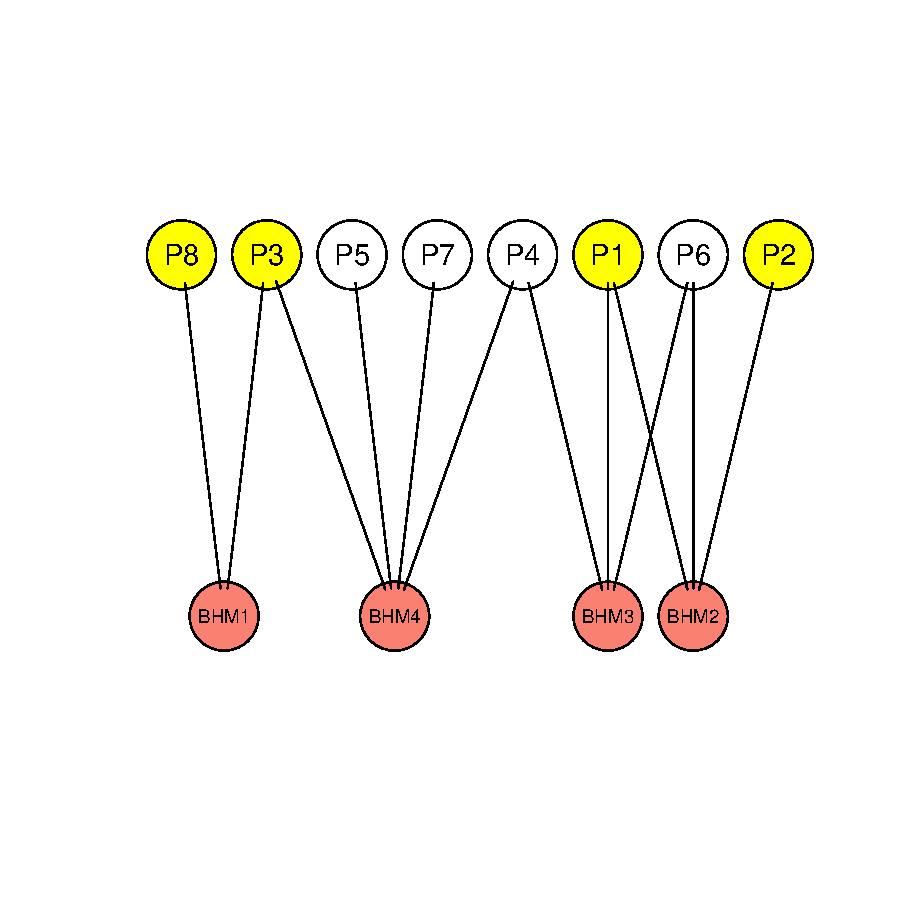
\includegraphics[width=0.5\textwidth]{apComplex-BP1}
\caption{\label{fig:BP1} Bipartite PCMG for the initial complex estimates
determined by locating maximal BH-complete subgraphs in the graph of observed AP-MS data.}
\end{center}
\end{figure}

The initial maximal BH-complete subgraph estimate of the PCMG does not allow missing
edges between bait and hit-only proteins; since AP-MS technology
is not perfectly sensitive, it is reasonable to expect a number of missing
edges in the subgraph for each complex estimate.  \Rpackage{apComplex}
accommodates this by employing an objective function to evaluate the complex
estimates.  For a complex $c_k$, let $C(c_k)$
represent the product of 1) the binomial
probability for the number of observed edges in $c_k$ given the number
of tested edges, and 2) a two-sided $p$-value from Fisher's exact test for the
distribution of missing incoming edges for complex estimate $c_k$.  Then let
$C$ equal the product of $C(c_k)$ over all complexes $c_1,...,c_K$.  The objective function
$P$ is the product of $L$ and $C$, or $P=L \times C$.  $L$ is maximized with
the initial maximal BH-complete subgraphs -- the algorithm in
\Rpackage{apComplex} looks to increase $C$ in favor of small decreases in $L$.

After the initial PCMG estimate is made using \Rfunction{bhmaxSubgraph},
\Rfunction{mergeComplexes} proposes pairwise unions of individual complex estimates.  If $P$ increases when the complexes are treated
as one, then the combination is accepted.  If more than one union increases
$P$, then the union with the largest increase is accepted.  Algebraic details
of the acceptance criteria are available in Scholtens and Gentleman (2004).

\begin{Schunk}
\begin{Sinput}
> PCMG1 <- mergeComplexes(PCMG0, apEX, sensitivity = 0.7, specificity = 0.75)
> PCMG1
\end{Sinput}
\begin{Soutput}
   Complex1 Complex2 Complex3
P1        0        1        0
P2        0        1        0
P3        1        0        1
P8        1        0        0
P4        0        1        1
P5        0        0        1
P6        0        1        0
P7        0        0        1
\end{Soutput}
\end{Schunk}

In this case, \Robject{bhmax2} and \Robject{bhmax3} were combined
into \Robject{Complex2}. (\Robject{bhmax1} and \Robject{bhmax4} remained as
originally estimated and are now named
\Robject{Complex1} and \Robject{Complex3}, respectively).  The one
missing edge out of the six tested in \Robject{Complex2} is consistent with the sensitivity of the
technology and the distribution of missing edges (in this case only one) is sufficiently random in the
subgraph for \Robject{Complex2}.  Figure \ref{fig:mergedComplex} contains the subgraphs for the
new complex estimates and Figure \ref{fig:BP2} shows the corresponding bipartite PCMG.


\begin{figure}[htbp]
\begin{center}
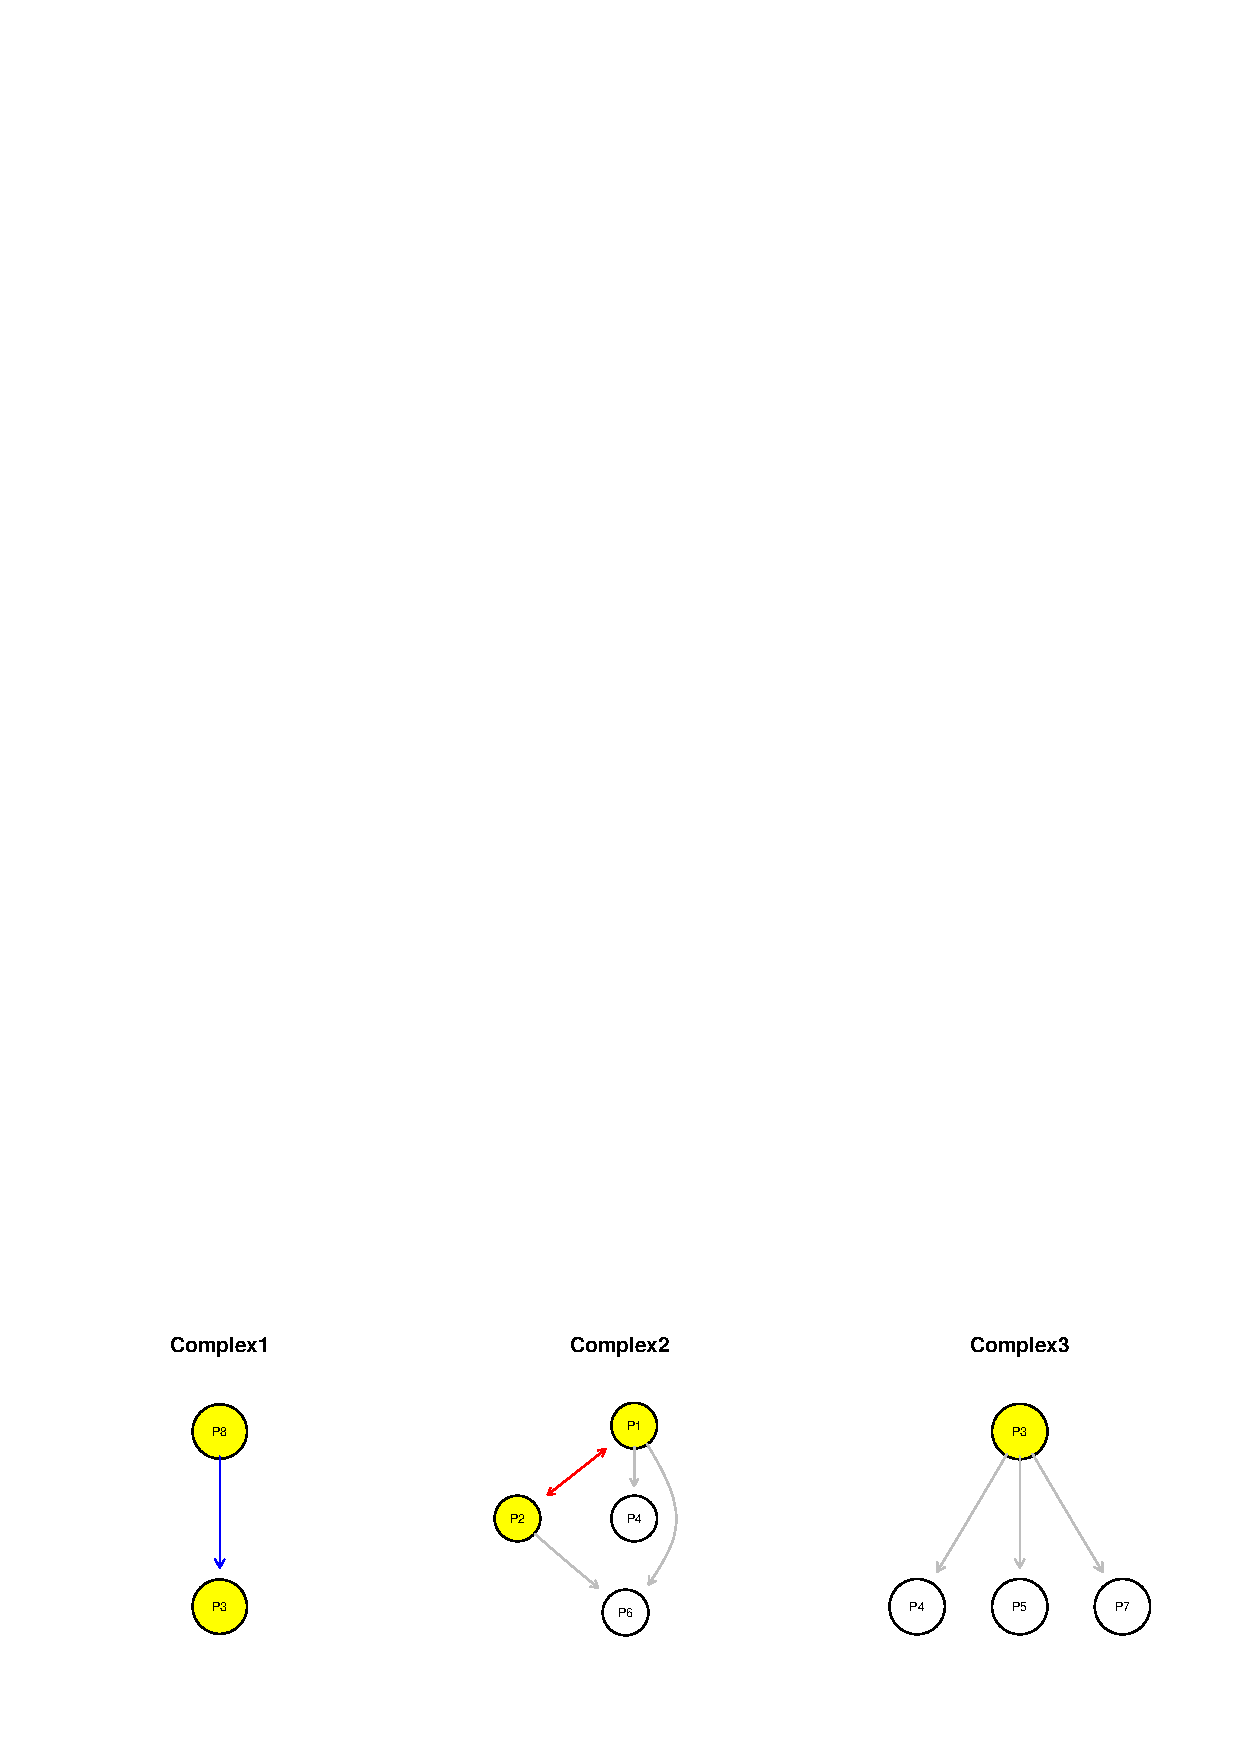
\includegraphics[width=0.75\textwidth]{apComplex-mergedComplex}
\caption{\label{fig:mergedComplex} Subgraphs for new complex estimates after
using \Rfunction{mergeComplexes}.}
\end{center}
\end{figure}


\begin{figure}[htbp]
\begin{center}
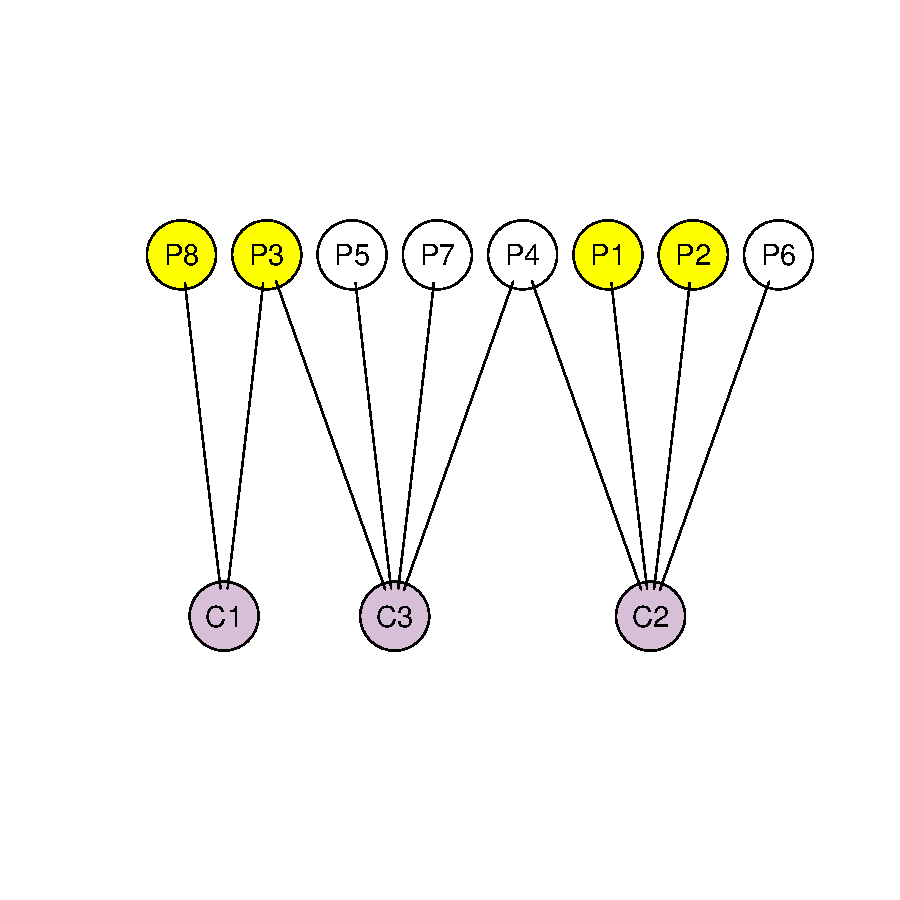
\includegraphics[width=0.5\textwidth]{apComplex-BP2}
\caption{\label{fig:BP2}Bipartite graph for new complex estimates after using
\Rfunction{mergeComplexes}.}
\end{center}
\end{figure}

The function \Rfunction{findComplexes} can be used to run both steps together.

\begin{Schunk}
\begin{Sinput}
> PCMG2 <- findComplexes(apEX, sensitivity = 0.7, specificity = 0.75)
\end{Sinput}
\begin{Soutput}
[1] "Finding Initial Maximal BH-complete Subgraphs"
[1] "Combining Complex Estimates"
\end{Soutput}
\begin{Sinput}
> PCMG2
\end{Sinput}
\begin{Soutput}
   Complex1 Complex2 Complex3
P1        0        1        0
P2        0        1        0
P3        1        0        1
P8        1        0        0
P4        0        1        1
P5        0        0        1
P6        0        1        0
P7        0        0        1
\end{Soutput}
\end{Schunk}

Our algorithm makes three types of complex estimates: multi-bait-mult-edge
(MBME) complexes that contain multiple baits and multiple edges,
single-bait-multi-hit (SBMH) complexes that contain a single bait and a
collection of hit-only proteins, and unreciprocated bait-bait (UnRBB)
complexes that only contain two bait proteins connected by one unreciprocated
edge.  MBME complexes are the most reliable outputs since they contain the
most tested data.  SBMH complexes are useful for proposing future experiments
since the topology among the hit-only proteins is unknown.  UnRBB complexes
may result from FP observations since the edges are tested twice, observed once, and
not confirmed by other subgraph edges.  On the other hand, the unreciprocated
edge may also result from a FN observation between the two baits.  The PCMG
affiliation matrix resulting from \Rfunction{mergeComplexes} or
\Rfunction{findComplexes} can be
sorted into the MBME, SBMH, and UnRBB components using the function
\Rfunction{sortComplexes}.

\begin{Schunk}
\begin{Sinput}
> sortComplexes(PCMG2, adjMat = apEX)
\end{Sinput}
\begin{Soutput}
$MBME
   MBME1
P1     1
P2     1
P3     0
P8     0
P4     1
P5     0
P6     1
P7     0

$SBMH
   SBMH1
P1     0
P2     0
P3     1
P8     0
P4     1
P5     1
P6     0
P7     1

$UnRBB
   UnRBB1
P1      0
P2      0
P3      1
P8      1
P4      0
P5      0
P6      0
P7      0
\end{Soutput}
\end{Schunk}

Recall that the true complexes in this example consist of $P_{1}$, $P_{2}$,
$P_{4}$, and $P_{6}$ and $P_{3}$, $P_{4}$, and $P_{5}$.  \Robject{MBME1}
accurately estimates $P_{1}$, $P_{2}$, $P_{4}$, and $P_{6}$ as composing one
complex.  \Robject{SBMH1} predicts $P_{3}$, $P_{4}$, and $P_{5}$ as members of
one complex, but also includes the FP observation for $P_{7}$.  The limited
data for this complex makes it impossible to distinguish the FP from the true
positive (TP) observations.  Further purifications using $P_{4}$, $P_{5}$, and
$P_{7}$ as baits would likely resolve this difficulty.  \Robject{UnRBB1} is
the result of the FP observation between $P_{8}$ and $P_{3}$. While it is
reported as a complex estimate, further experimental testing would likely
confirm that this is not a true complex.

If the user desires, a matrix of similarity data can be included as the
\Robject{simMat} argument in \Rfunction{mergeComplexes} and
\Rfunction{findComplexes} in an extended logistic regression model.  The
similarity measure can be used to lend credence to the existence of an edge,
even if it is not detected using AP-MS.  Users
must specify the parameter \Robject{Beta} which weights contribution of the
similarity measure to the model.  See Scholtens and Gentleman (2004) for
details.

\section*{Publicly available data}

Two publicly available data sets are included in \Rpackage{apComplex}.
\Robject{TAP} is an adjacency matrix of the AP-MS data (called `TAP') reported by Gavin, et
al. (2002).  There were 3420 comemberships reported using 455 baits and 909
hit-only proteins.  \Robject{TAPgraph} contains a graph of class
\Robject{graphNEL} of the TAP data.  The TAP data were originally compiled
into 232 yTAP complexes, available in Supplementary Table 1 of Gavin, et
al. (2002) at http://www.nature.com and at http://yeast.cellzome.com.  These
yTAP complex estimates, along with the annotations given by Gavin, et al. are
available in \Robject{yTAP}.  

\begin{Schunk}
\begin{Sinput}
> data(TAP)
> dim(TAP)
\end{Sinput}
\begin{Soutput}
[1]  455 1364
\end{Soutput}
\begin{Sinput}
> data(TAPgraph)
> TAPgraph
\end{Sinput}
\begin{Soutput}
A graph with  directed  edges
Number of Nodes = 1364
Number of Edges = 3420
\end{Soutput}
\begin{Sinput}
> which(TAP["Abd1", ] == 1)
\end{Sinput}
\begin{Soutput}
Rpb2 Spt5 
 926 1049 
\end{Soutput}
\begin{Sinput}
> adj(TAPgraph, "Abd1")
\end{Sinput}
\begin{Soutput}
$Abd1
[1] "Rpb2" "Spt5"
\end{Soutput}
\begin{Sinput}
> data(yTAP)
> yTAP[1]
\end{Sinput}
\begin{Soutput}
$yTAPC1
$yTAPC1$proteins
[1] "Tfc1" "Itc1" "Tfc3" "Tfc4" "Tfc6" "Tfc7" "Tfc8"

$yTAPC1$yTAPfunction
[1] "Transcription/DNA maintenance/chromatin structure"
\end{Soutput}
\end{Schunk}

\Robject{HMSPCI} is an adjacency matrix of the AP-MS data (called `HMS-PCI') reported by Ho, et
al. (2002).  There were 3687 comemberships reported using 493 baits and 1085
hit-only proteins.  \Robject{HMSPCIgraph} contains a graph of class
\Robject{graphNEL} of the HMS-PCI data.  

\begin{Schunk}
\begin{Sinput}
> data(HMSPCI)
> dim(HMSPCI)
\end{Sinput}
\begin{Soutput}
[1]  493 1578
\end{Soutput}
\begin{Sinput}
> data(HMSPCIgraph)
> HMSPCIgraph
\end{Sinput}
\begin{Soutput}
A graph with  directed  edges
Number of Nodes = 1578
Number of Edges = 3687
\end{Soutput}
\begin{Sinput}
> which(HMSPCI["YAL015C", ] == 1)
\end{Sinput}
\begin{Soutput}
YDL029W YJR068W YMR146C YPR110C YDR214W YEL030W YEL060C YMR012W YMR058W YNL037C 
     62     280     367     488     704     759     765    1274    1279    1333 
\end{Soutput}
\begin{Sinput}
> adj(HMSPCIgraph, "YAL015C")
\end{Sinput}
\begin{Soutput}
$YAL015C
 [1] "YDL029W" "YJR068W" "YMR146C" "YPR110C" "YDR214W" "YEL030W" "YEL060C"
 [8] "YMR012W" "YMR058W" "YNL037C"
\end{Soutput}
\end{Schunk}

These data were analyzed using \Rpackage{apComplex}, and the results are
described in Scholtens, Vidal, and Gentleman
(submitted).  The complex estimates are available for both data sets -
\Robject{MBMEcTAP}, \Robject{SBMHcTAP}, and \Robject{UnRBBcTAP} for the TAP
data, and \Robject{MBMEcHMSPCI}, \Robject{SBMHcHMSPCI}, and
\Robject{UnRBBcHMSPCI} for the HMS-PCI data.  

One example of the detail with which the \Rpackage{apComplex} algorithm can
estimate complex membership involves the PP2A proteins Tpd3, Cdc55, Rts1,
Pph21, and Pph22.  These five proteins compose four heterotrimers (Jiang and
Broach, 1999).  We
accurately predict these trimers as distinct complexes. and furthermore note
the exclusive association of Zds1 and Zds2 with the Cdc55/Pph22 trimer.
Confirmation of this prediction in the lab may help clarify the cellular
function of this particular trimer and the reason for its joint activity with
Zds1 and Zds2.

\begin{Schunk}
\begin{Sinput}
> data(MBMEcTAP)
> which(MBMEcTAP[, 37] == 1)
\end{Sinput}
\begin{Soutput}
Cdc55 Pph22  Tpd3  Zds2 
   48   219   369   454 
\end{Soutput}
\begin{Sinput}
> which(MBMEcTAP[, 38] == 1)
\end{Sinput}
\begin{Soutput}
Cdc55 Pph22  Tpd3  Zds1 
   48   219   369   453 
\end{Soutput}
\begin{Sinput}
> which(MBMEcTAP[, 39] == 1)
\end{Sinput}
\begin{Soutput}
Cdc55  Tpd3 Pph21 
   48   369   858 
\end{Soutput}
\begin{Sinput}
> which(MBMEcTAP[, 195] == 1)
\end{Sinput}
\begin{Soutput}
Pph22  Rts1  Tpd3 
  219   286   369 
\end{Soutput}
\begin{Sinput}
> which(MBMEcTAP[, 233] == 1)
\end{Sinput}
\begin{Soutput}
 Rts1  Tpd3 Pph21 
  286   369   858 
\end{Soutput}
\end{Schunk}

In summary, \Rpackage{apComplex} can be used to predict complex membership
using data from AP-MS experiments.  An accurate catalog of complex membership
is a fundamental requirement for understanding functional modules in the cell.  Integration of \Rpackage{apComplex} analyses with other
high-throughput data, including binary physical interactions assayed by
yeast two-hybrid technology, gene expression data, and binding domain data
are promising avenues for further systems biology research.

\section*{References}

\noindent Gavin, A.-C., et al. (2002) Functional organization of the yeast
proteome by systematic analysis of protein complexes, \textit{Nature},
\textbf{415}, 141-147.

\vspace{.2in}

\noindent Ho, Y., et al. (2002) Systematic identification of protein complexes
in \textit{Saccharomyces cerevisiae} by mass spectrometry,
\textit{Nature}. \textbf{415}, 180-183.

\vspace{.2in}

\noindent Jiang, Y., Broach, J. (1999) Tor proteins and protein phosphatase
2A reciprocally regulate Tap42 in controlling cell growth in yeast,
\textit{EMBO Journal}, \textbf{18}, 2782-2792.

\vspace{.2in}

\noindent Scholtens, D., Gentleman, R. (2004) Making sense of high-throughput
protein-protein interaction data, \textit{Statistical Aplications in Genetics
and Molecular Biology}, \textbf{3}, Article 39.

\vspace{.2in}

\noindent Scholtens, D., Vidal, M., Gentleman, R.  Local modeling of global
interacome networks, \textit{Submitted}.

\end{document}
